\documentclass[a4paper, fontsize=11pt]{scrartcl} % A4 paper and 11pt font 
\usepackage[a4paper,left=3cm,right=2cm,top=2.5cm,bottom=2.5cm]{geometry}

\usepackage[T1]{fontenc} % Use 8-bit encoding that has 256 glyphs
\usepackage{fourier} % Use the Adobe Utopia font for the document - comment this line to return to the LaTeX default
\usepackage[spanish]{babel} % Spanish language/hyphenation
\selectlanguage{spanish}
\usepackage[utf8]{inputenc}
\usepackage{amsmath,amsfonts,amsthm} % Math packages
\usepackage{graphicx} % The graphicx package
\usepackage{placeins}
\usepackage{caption}
\usepackage{subcaption}


\usepackage{listings} % Insert Scripts
\usepackage{color} %red, green, blue, yellow, cyan, magenta, black, white
\definecolor{mygreen}{RGB}{28,172,0} % color values Red, Green, Blue
\definecolor{mylilas}{RGB}{170,55,241}

\lstset{language=Matlab,%
	%basicstyle=\color{red},
	breaklines=true,%
	morekeywords={matlab2tikz},
	keywordstyle=\color{blue},%
	morekeywords=[2]{1}, keywordstyle=[2]{\color{black}},
	identifierstyle=\color{black},%
	stringstyle=\color{mylilas},
	commentstyle=\color{mygreen},%
	showstringspaces=false,%without this there will be a symbol in the places where there is a space
	numbers=left,%
	numberstyle={\tiny \color{black}},% size of the numbers
	numbersep=9pt, % this defines how far the numbers are from the text
	emph=[1]{for,end,break},emphstyle=[1]\color{red}, %some words to emphasise
	%emph=[2]{word1,word2}, emphstyle=[2]{style},    
}

\usepackage{sectsty} % Allows customizing section commands
%\allsectionsfont{\centering \normalfont\scshape} % Make all sections centered, the default font and small caps

\usepackage{fancyhdr} % Custom headers and footers
\pagestyle{fancyplain} % Makes all pages in the document conform to the custom headers and footers
\fancyhead{} % No page header - if you want one, create it in the same way as the footers below
\fancyfoot[L]{} % Empty left footer
\fancyfoot[C]{} % Empty center footer
\fancyfoot[R]{\thepage} % Page numbering for right footer
\renewcommand{\headrulewidth}{0pt} % Remove header underlines
\renewcommand{\footrulewidth}{0pt} % Remove footer underlines
\setlength{\headheight}{13.6pt} % Customize the height of the header

\numberwithin{equation}{section} % Number equations within sections (i.e. 1.1, 1.2, 2.1, 2.2 instead of 1, 2, 3, 4)
\numberwithin{figure}{section} % Number figures within sections (i.e. 1.1, 1.2, 2.1, 2.2 instead of 1, 2, 3, 4)
\numberwithin{table}{section} % Number tables within sections (i.e. 1.1, 1.2, 2.1, 2.2 instead of 1, 2, 3, 4)

%\setlength\parindent{0pt} % Removes all indentation from paragraphs - comment this line for an assignment with lots of text

\newenvironment{myalign}{\par\nobreak\large\noindent\align}{\endalign} %Altering fontsize in equations globally

%----------------------------------------------------------------------------------------
%	TITLE SECTION
%----------------------------------------------------------------------------------------

\newcommand{\horrule}[1]{\rule{\linewidth}{#1}} % Create horizontal rule command with 1 argument of height

\title{	
	\normalfont \normalsize 
	\textsc{Master en Automática y Robótica - UPM} \\ [25pt] % Your university, school and/or department name(s)
	\horrule{0.5pt} \\[0.4cm] % Thin top horizontal rule
	\huge Control de Estructura Variable \\ % The assignment title
	\horrule{2pt} \\[0.5cm] % Thick bottom horizontal rule
}

\author{Jorge Camarero Vera - 07052} % Your name

\date{\normalsize\today} % Today's date or a custom date

\begin{document}
	\maketitle
	
	\section{Explicación de la tarea}
	
	La finalidad de esta tarea es aplicar un control de estructura variable a un modelo que el alumno escoja.
	
	\subsection{Desarrollo de la tarea}
	
	\subsubsection{Desarrollo del Modelo}
	
	Se ha escogido como modelo a controlar un \textbf{motor de corriente continua}, Figura \ref{Motor}.
	
	\begin{figure}[h!]
		\centering
		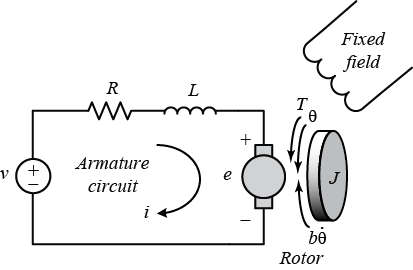
\includegraphics[width=0.8\linewidth]{images/motor.png}
		\caption{Motor de corriente continua.}
		\label{Motor}
	\end{figure}
	\FloatBarrier
	%
	Los parámetros físicos para este tipo de motor son:
	\begin{description}
	\item[Momento de inercia del rotor ($J$)] $0.01\,kg\cdot m^2$
	\item[Constante de fricción viscosa del motor ($b$)] $0.1\,N\cdot m\cdot s$
	\item[Constante de fuerza electromotriz ($K_e$)] $0.01\,\dfrac{V}{rad/sec}$
	\item[Constante de par del motor ($K_t$)] $0.01\,\dfrac{N\cdot m }{Amp}$
	\item[Resistencia eléctrica ($R$)] $1\,Ohm$
	\item[Inductancia electrica ($L$)] $0.5\,H$
	\end{description}
	
	La función de transferencia de este motor es la siguiente:
	
	\begin{myalign}
	P(S)=\dfrac{\dot{\theta}(s)}{V(s)}=\dfrac{K}{(Js+b)(Ls+R)+K^2} \qquad  \left[ \dfrac{rad/sec}{V} \right]
	\end{myalign}
	
	Lo pasamos a sistema del espacio de estados en Matlab:
	
	\begin{lstlisting}
	J = 0.01;
	b = 0.1;
	K = 0.01;
	R = 1;
	L = 0.5;
	s = tf('s');
	P_motor = K/((J*s+b)*(L*s+R)+K^2)
	
	P_motor =
	
		0.01
	---------------------------
	0.005 s^2 + 0.06 s + 0.1001
	
	num = 0.01;
	den = [0.005 0.06 0.1001];
	
	[A B C D] = tf2ss(num, den);
	sys = ss(A,B,C,D)
	
	sys =
	
	a = 
	x1      x2
	x1     -12  -20.02
	x2       1       0
	
	b = 
	u1
	x1   1
	x2   0
	
	c = 
	x1  x2
	y1   0   2
	
	d = 
	u1
	y1   0
	
	Continuous-time state-space model.
	
	\end{lstlisting}
	
	Con este modelo se lleva a Simulink y se cierra el bucle, Figura \ref{SimModel}, obteniéndose en la simulación ante un escalón unitario la salida de la Figura \ref{Output}.
	
	\begin{figure}[h!]
		\centering
		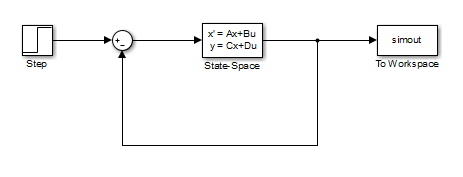
\includegraphics[width=1.0\linewidth]{images/SimModel.png}
		\caption{Modelo en Simulink del motor con el bucle cerrado.}
		\label{SimModel}
	\end{figure}
	\FloatBarrier
	
	\begin{figure}[h!]
		\centering
		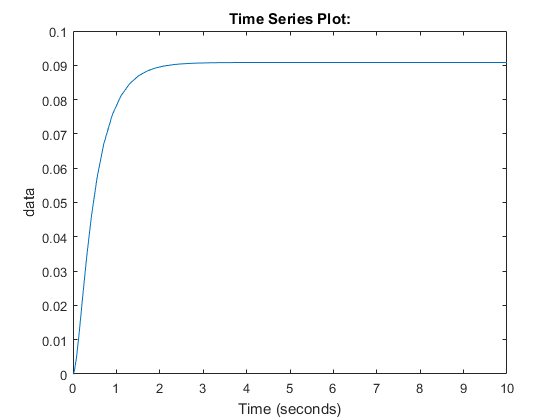
\includegraphics[width=0.8\linewidth]{images/Output.png}
		\caption{Motor de corriente continua.}
		\label{Output}
	\end{figure}
	\FloatBarrier
	
	\subsubsection{Desarrollo del Controlador de Estructura Variable}
	
	El modelo obtenido anteriormente pasado a canónica es:
	
	\[
	\begin{bmatrix}
	\dot{x}_1\\
	\dot{x}_2
	\end{bmatrix}
	=
	\begin{bmatrix}
	-12 & -20.02\\
	  1 &   0
	\end{bmatrix}
	\begin{bmatrix}
	x_1\\
	x_2
	\end{bmatrix}
	+
	\begin{bmatrix}
	1\\
	0
	\end{bmatrix}
	u
	\]
	\[
	y=
	\begin{bmatrix}
	0 & 2
	\end{bmatrix}
	\begin{bmatrix}
	x_1\\
	x_2
	\end{bmatrix}
	\]
	
	Escribiéndolo en forma de ecuaciones:
	\begin{myalign}
		\begin{split}
			\dot{x}_2 &= x_1\\
			\dot{x}_1 &= -12\cdot x_1-20.02\cdot x_2+u
		\end{split}
	\end{myalign}
	
	Con la línea de conmutación, $s = c \cdot x_1 + x_2$, y su derivada, $s = x \cdot \dot{x}_1 + \dot{x}_2$, hay que definir la ley de control $u$:
	\begin{myalign}
		u = REF - \Psi x_1
	\end{myalign}
	%
	Donde: 
	
	\[ \Psi =
	\begin{cases}
	\alpha &  si x_1\cdot s<0\\
	\beta  &  si x_1\cdot s>0\\
	\end{cases}
	\]
	
	Sustituyendo las expresiones anteriores, se obtiene:
	
	\begin{myalign}
		\dot{s} = 12 \cdot x_2 - 20.02 \cdot c \cdot x_2 + c \cdot u - \dfrac{x_2}{c}
	\end{myalign}
	
	Si se toma $REF$ entonces $u=-\Psi \cdot x_2$, quedando:
	\begin{myalign}
		\dot{s} = \left( 12 -20.02\cdot - \dfrac{1}{c} - \Psi \cdot c \right)  \cdot x_2
	\end{myalign}
	
	Como $s \cdot x_1 < 0$ entonces queda que:
	
	\begin{myalign}
		\Psi = \dfrac{12}{c} -20.02 - \dfrac{1}{c^2}
	\end{myalign}
	
	Planteamos el sistema en Simulink, Figura \ref{VSC1} y obtenemos la salida ante $T = 2$, Figura \ref{Output1}.
	
	\begin{figure}[h!]
		\centering
		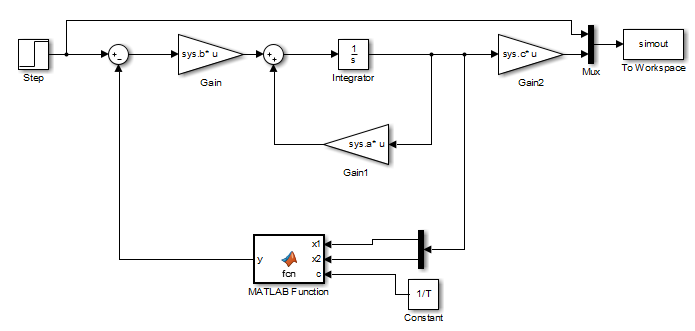
\includegraphics[width=0.8\linewidth]{images/SimModel_VSC.png}
		\caption{Modelo con la implementación del Control de Estructura Variable.}
		\label{VSC1}
	\end{figure}
	\FloatBarrier
	
	El script planteado en la función de Matlab en Simulink es la siguiente:
	
	\begin{lstlisting}
	function y = fcn(x1,x2,c)
	
	Psi = 12/c - 20.02 - 1/c^2;
	s = c * x1 + x2;
	if s * x2 > 0
		x2 = x2 * Psi;
	else
		x2 = -x2 * Psi;
	end
	
	y = x2;
	\end{lstlisting}
	
	\begin{figure}[h!]
		\centering
		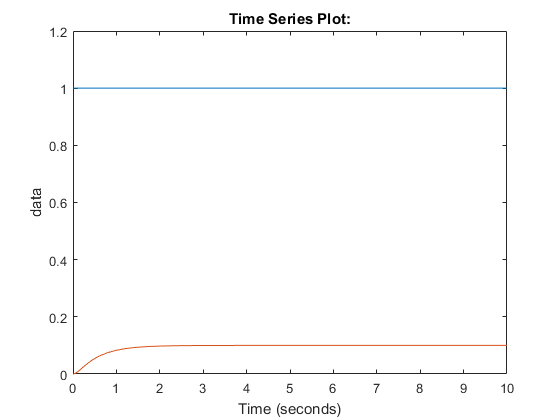
\includegraphics[width=0.8\linewidth]{images/Output1.png}
		\caption{Salida controlada mediante Control de Estructura Variable.}
		\label{Output1}
	\end{figure}
	\FloatBarrier
	
	\subsubsection{Caso con otro modelo del espacio de estados.}
	
	En el caso anteriormente propuesto se ha hecho para la condición $s \cdot x_2 > 0$, esta vez se quiere para $s \cdot x_1 > 0$, por lo que el modelo de estados habrá que plantearlo de manera distinta.\\
	
	\begin{lstlisting}
	Ap = [0 1; -20.02 -12]
	Bp = [0; 2]
	Cp = [1 0]
	
	sys_p = ss(Ap,Bp,Cp,0)
	
	sys_p =
	
	a = 
	x1      x2
	x1       0       1
	x2  -20.02     -12
	
	b = 
	u1
	x1   0
	x2   2
	
	c = 
	x1  x2
	y1   1   0
	
	d = 
	u1
	y1   0
	
	Continuous-time state-space model.
	\end{lstlisting}
	
	Escrito de otra forma:
	
	\[
	\begin{bmatrix}
		\dot{x}_1\\
		\dot{x}_2
	\end{bmatrix}
	=
	\begin{bmatrix}
		0 & 1\\
		-20.02 &   -12
	\end{bmatrix}
	\begin{bmatrix}
		x_1\\
		x_2
	\end{bmatrix}
	+
	\begin{bmatrix}
		0\\
		2
	\end{bmatrix}
	u
	\]
	\[
	y=
	\begin{bmatrix}
	1 & 0
	\end{bmatrix}
	\begin{bmatrix}
	x_1\\
	x_2
	\end{bmatrix}
	\]
	%
	Teniendo $s = c \cdot x_1 + x_2$ y su derivada, $\dot{s} = c \cdot \dot{x}_1 + \dot{x}_2$, y con:
	
	\begin{myalign}
		\begin{split}
			\dot{x}_1 &= x_2 \\
			\dot{x}_2 &= -20.02 \cdot x_1 - 12 \cdot x_2 + 2 \cdot u
		\end{split}
	\end{myalign}
	%
	Se obtiene sustituyendo entre sí:
	
	\begin{myalign}
		\dot{s} = -c^2 \cdot x_1 + 12 \cdot c \cdot x_1 - 20.02 \cdot x_1 + 2 \cdot u
	\end{myalign}
	%
	Y conociendo que $u = - \Psi \cdot x_1$, sustituyendo se llega a:
	
	\begin{myalign}
		\Psi = \dfrac{c^2}{2} + 6 \cdot c - 10.01
	\end{myalign}
	
	Se plantea el sistema en Simulink, Figura \ref{VSC2}, y se obtiene la salida para $T = 2$, Figura \ref{Output2}.\\
	
	\begin{figure}[h!]
		\centering
		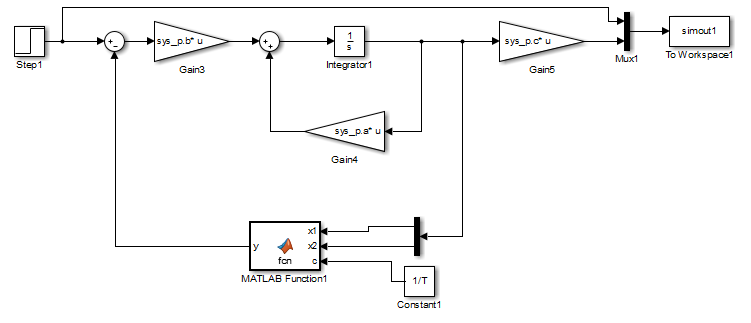
\includegraphics[width=0.8\linewidth]{images/SimModel_VSC1.png}
		\caption{Modelo con la implementación del Control de Estructura Variable.}
		\label{VSC2}
	\end{figure}
	\FloatBarrier
	
	El script planteado en la función de Matlab en Simulink es la siguiente:
	
	\begin{lstlisting}
	function y = fcn(x1,x2,c)
	
	Psi = ((c^2)/2 + 6*c - 10.01);
	s = c * x1 + x2;
	if (s * x1) > 0
		x1 = x1 * Psi;
	else
		x1 = -x1 * Psi;
	end
	
	y = x1;
	\end{lstlisting}
		
	\begin{figure}[h!]
		\centering
		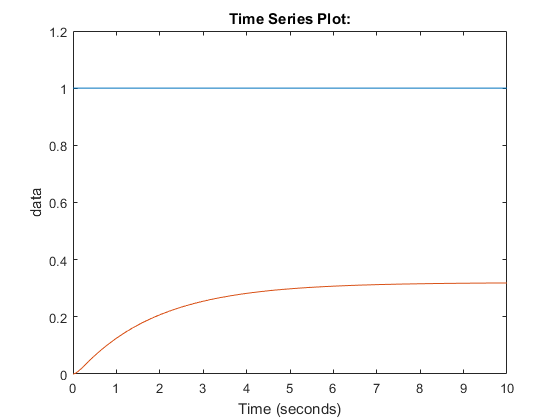
\includegraphics[width=0.8\linewidth]{images/Output2.png}
		\caption{Salida controlada mediante Control de Estructura Variable.}
		\label{Output2}
	\end{figure}
	\FloatBarrier
	%
	
	\begin{figure}[h!]
		\centering
		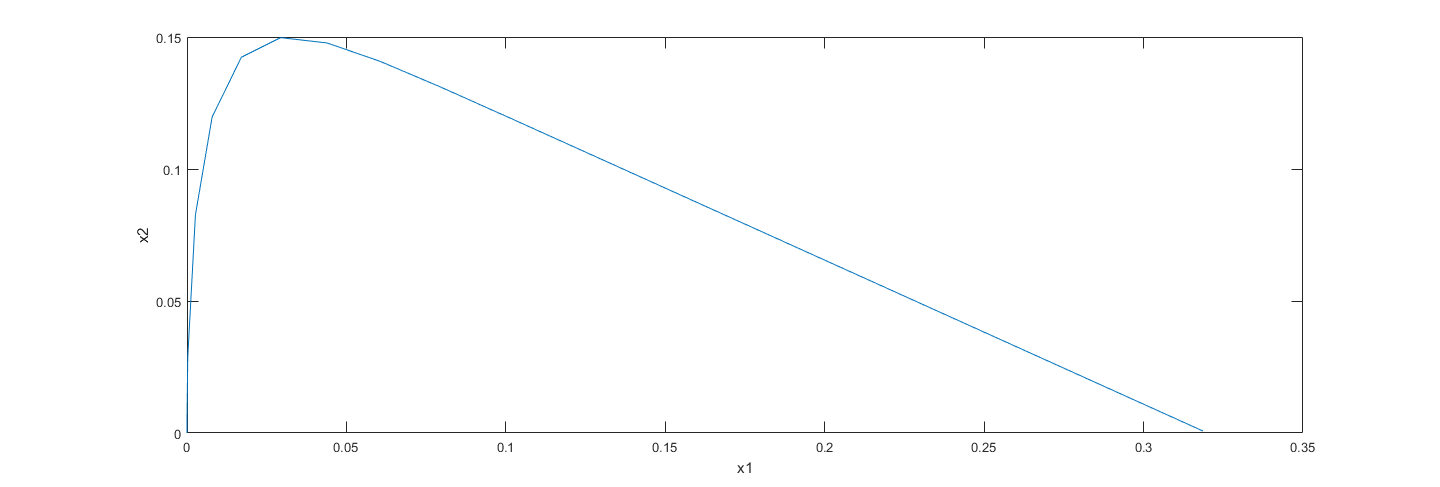
\includegraphics[width=1.0\linewidth]{images/states.png}
		\caption{Espacio de Estados}
		\label{States}
	\end{figure}
	\FloatBarrier
	%
	Y comparamos la salida de los estados $x1$ y $x2$ en la Figura \ref{States}.
	
\end{document}